\section{SSSP (Single Source Shortest Path)}
\subsection{Dijkstra}
\begin{frame}
\frametitle{Das Problem}
\begin{block}{Das Problem}
Breitensuche schlägt bei gewichteten Graphen fehl: 

\begin{figure}
\includegraphics[scale=.75]{dijkstra_graphs/bfs_fail_0.pdf}
\end{figure}

\end{block}
\end{frame}

\begin{frame}
\frametitle{Das Problem}
\begin{figure}
\includegraphics[scale=.8]{dijkstra_graphs/bfs_fail_0.pdf}
\end{figure}
\end{frame}

\begin{frame}
\frametitle{Das Problem}
\begin{figure}
\includegraphics[scale=.8]{dijkstra_graphs/bfs_fail_1.pdf}
\end{figure}
\end{frame}

\begin{frame}
\frametitle{Das Problem}
\begin{figure}
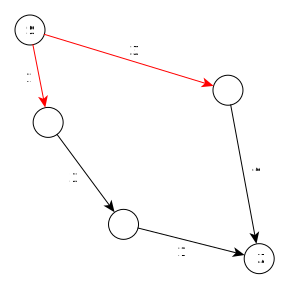
\includegraphics[scale=.8]{dijkstra_graphs/bfs_fail_2.pdf}
\end{figure}
\end{frame}

\begin{frame}
\frametitle{Das Problem}
\begin{figure}
\includegraphics[scale=.8]{dijkstra_graphs/bfs_fail_3.pdf}
\end{figure}
\end{frame}

\begin{frame}
\frametitle{Das Problem}
\begin{figure}
\includegraphics[scale=.8]{dijkstra_graphs/bfs_fail_4.pdf}
\end{figure}
\end{frame}

\begin{frame}
\frametitle{Das Problem}
\begin{figure}
\includegraphics[scale=.8]{dijkstra_graphs/bfs_fail_4.pdf}
\end{figure}

$\implies$ Es wird ein Weg der Länge $7$ gefunden, obwohl $5$ das Optimum ist

\end{frame}


\begin{frame}
\frametitle{Djikstras Algorithmus}
\begin{itemize}
\item Grundsätzliche Idee: Breitensuche mit Priortiy-Queue (so dass "nähere" Knoten zuerst behandelt werden)
\item Dynamic Programming um doppeltes Untersuchen von Knoten zu vermeiden. 
\item \lstinline|std::priority_queue| verwendet binären Heap
\item $\implies$ Laufzeit von Dijkstra ist $\Theta((|E| + |V|) \log |V|)$
\item Theoretisch mit Fibonacci-Heap bessere Laufzeit, aber \begin{itemize}
\item Praktisch langsamer für ICPC-Problemgrößen
\item Und dann auch nur bei sehr dichten Graphen
\item Nicht in der C++-Standardbibliothek
\end{itemize}
\end{itemize}
\end{frame}

\begin{frame}[fragile]
\frametitle{Code}
Header: 
\begin{lstlisting}[basicstyle=\tiny]
#include<vector>
#include<algorithm>
#include<queue> 
#include<iostream>

using namespace std;

struct edge {
    size_t to;
    double weight;
};

bool operator < (const edge& e1, const edge& e2) {
    // inversed, because priority_queue returns biggest element
    return e1.weight > e2.weight;
}

using node = vector<edge>;
\end{lstlisting}

\end{frame}

\begin{frame}[fragile]
\frametitle{Code}
\begin{lstlisting}[basicstyle=\tiny]
vector<double> dijkstra(vector<node>& nodes, size_t startnode) {
  // initialize all distances with infinity
  vector<double> distances (nodes.size(), 100000000000);

  priority_queue<edge> todo;

  todo.push({startnode, 0});
  
  while(!todo.empty()) {
    auto current = todo.top();
    todo.pop();

    if(current.weight < distances[current.to]) {
      distances[current.to] = current.weight;

      for(size_t i = 0; i < nodes[current.to].size(); i++) {
        edge next = nodes[current.to][i];
        next.weight += current.weight;

        todo.push(next);
      }
    }
  }

  return distances;
}
\end{lstlisting}

\end{frame}

\begin{frame}[fragile]
\frametitle{Code}
\begin{lstlisting}[basicstyle=\tiny]
int dijkstra_to_target(vector<node>& nodes, size_t startnode, size_t target) {
  vector<double> distances (nodes.size(), 100000000000);

  priority_queue<edge> todo;

  todo.push({startnode, 0});
  
  while(!todo.empty()) {
    auto current = todo.top();
    todo.pop();

    // Early return
    if(current.to == target) return current.weight;

    if(current.weight < distances[current.to]) {
      distances[current.to] = current.weight;

      for(size_t i = 0; i < nodes[current.to].size(); i++) {
        edge next = nodes[current.to][i];
        next.weight += current.weight;

        todo.push(next);
      }
    }
  }

  // target not found
  return -1;
}
\end{lstlisting}

\end{frame}